\section{Empirical Study} \label{sec:results}
We answer three research questions by analyzing Low Code Software Development (LCSD)  discussions in SO.
\begin{enumerate}[leftmargin=30pt, label=\bf{RQ\arabic{*}.}]
  \item What types of topics are discussed about LCSD? 
  \item How are the topics distributed across low-code SDLC? 
  \item What LCSD topics are the most difficult to answer?
  %\item How do the topics vary across the different low code software providers?
  %\item What types of questions are asked about low code software in Stack Overflow?
  %\item How do the popularity and difficulty of the topics vary in Stack Overflow?
  %\item How do the topics evolve over time in Stack Overflow?
\end{enumerate}
The first research question aims to understand the types of topics discussed in
SO about LCSD (\sec\ref{sec:rq-topic-type}). The second research
question aims to understand how each topic is discussed across different stages of low-code SDLC (software development life cycle) (\sec\ref{sec:rq-topic-challenges}). The third research question offers insight into the challenges of LCSD 
developers across the observed LCSD topics based on the measurement of difficulty of getting answers (\sec\ref{sec:rq-topic-difficulty}).


\subsection{What types of topics are discussed about LCSD? (RQ1)}\label{sec:rq-topic-type}

 

% \begin{figure}[htb]
% \centering
% 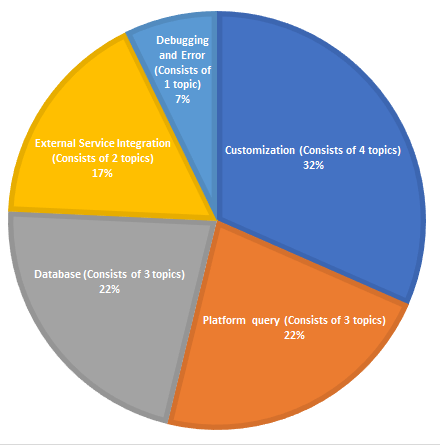
\includegraphics[scale=0.90]{res/PieChart.png}
% % 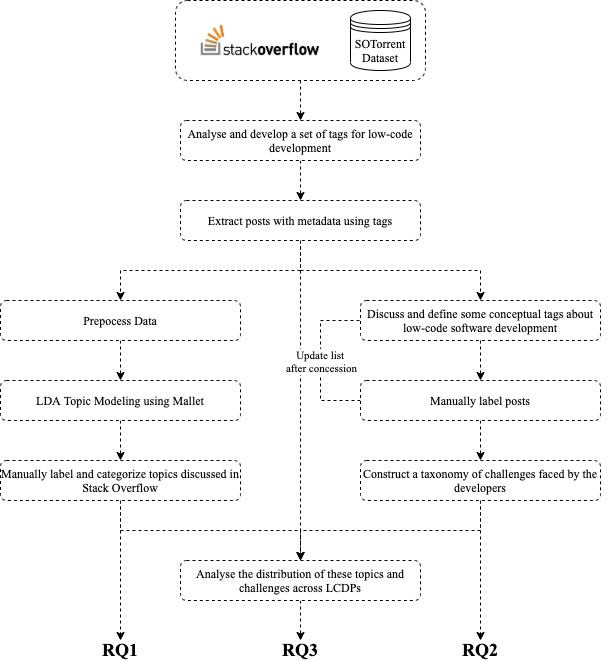
\includegraphics[width=0.35 * linewidth]{res/methology_overview.jpg}
% \caption{ Distribution of percentage of questions and topics per higher level category}
% \label{fig:distribution_of_questions_topic_pie_chart}
% \end{figure}
% \subsubsection{Motivation}
% Low-code software development is becoming more and more popular as a flexible
% and easy approach to develop useful business applications. In many ways low-code
% software development is different from traditional software development. Being a
% recent trend, the challenges of low-code development are yet to be studied well
% as observed in discussed in \sec\ref{sec:related_work}. SO is an established source of knowledge repository that can
% be used for the systematic study of the real world challenges faced by the
% practitioners. Hence, the low-code related SO data mined as described in Section
% \ref{sec:methodology} offers us the opportunity to analyze topics of discussions
% of the low-code practitioners. Investigating this first research question will
% help LCSD platform developers and researchers to have better understanding of
% prevalent issues and improve the quality of LCSD technology.

\subsubsection{Approach}
We get 13 low-code related topics from our LDA topic modeling as discussed in \sec\ref{sec:methodology}. We use card sorting \cite{fincher2005making} to label these topics  following previous
works \cite{bagherzadeh2019going, ahmed2018concurrency, yang2016security, rosen2016mobile, abdellatif2020challenges}.
In open card sorting, there is no predefined list of labels. To label a topics, 
we used the top 30 words for the topic and a random sample of at least 20 questions that are assigned to the topic. Four of the authors participated in the labelling process.
Each author assigns a label for each topic and discusses with each other until
there is an agreement. The authors reached an agreement after around 15
iterations of meetings over Skype and email and labeled the 13 topics from the
LDA output discussed in Section \ref{sec:background}. After the labeling of the topics, we grouped them into higher categories. For
example, UI Adaptation and Dynamic Form Controller are related to UI design, and
so we group them into a group named UI. In the same way, Dynamic Event Handling,
Dynamic Content Display, and Dynamic Content Binding topics are related to the
middleware feature of low-code development platforms, and so we put these three
topics into Middleware sub-category. We repeat these process until we can not
find any more higher-level group. For example, the above mentioned two
categories UI and Middleware belong to the application customization task where
the developers customize the UI or the business logic of the application
according to their need. Hence, we put them under a high-level category named
Customization. Similarly, we put Access Control \& Security into Configuration sub-category. Then we put Configuration sub-category and Client Server Comm \& IO topic under Platform Adaptation high-level category.

% Similarly, we put SQL CRUD into Management sub-category and Data
% Storage \& Migration to Migration sub-category and then put these two
% sub-categories under a higher category named Database.


\begin{figure}[t]
	\centering\begin{tikzpicture}[scale=0.28]-
    \pie[
        /tikz/every pin/.style={align=center},
        text=pin, number in legend,
        explode=0.0,
        color={black!0, black!10, black!20, black!30,, black!40},
        ]
        {
            17/\bf{Third-Party}\\Integration\\ (17\%Q 2T),
            40/\bf{Customization}\\UI or Service (40\%Q 5T),
            22/\bf{Platform}\\ Adoption (22\%Q 3T),
            22/\bf{Database}\\Management\\ (22\%Q 3T)
        }
    \end{tikzpicture}
	\caption{Distribution of questions (Q) and topics (T) per topic category}
	\vspace{-5mm}
	\label{fig:distribution_of_questions_topic_pie_chart}
\end{figure}

\begin{figure}[t]
\centering
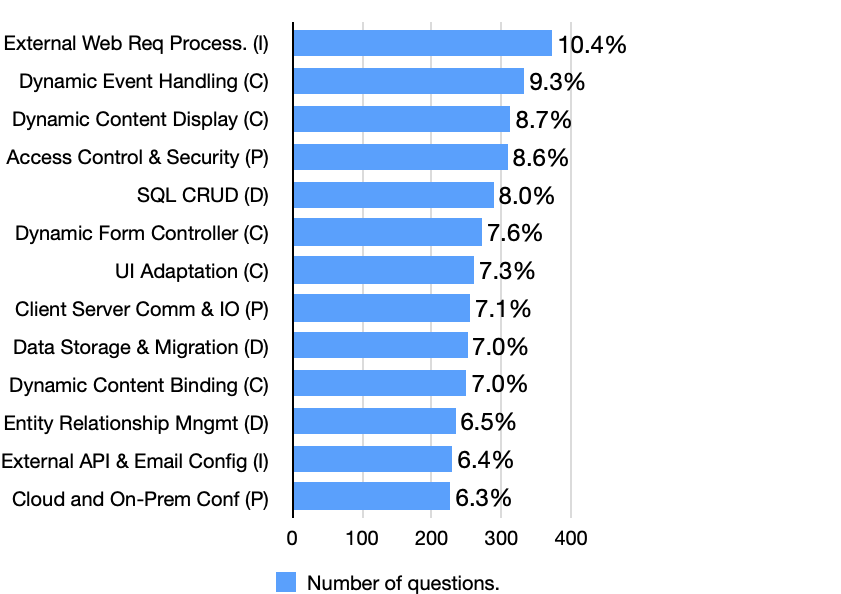
\includegraphics[scale=0.32]{res/barChart.png}
% 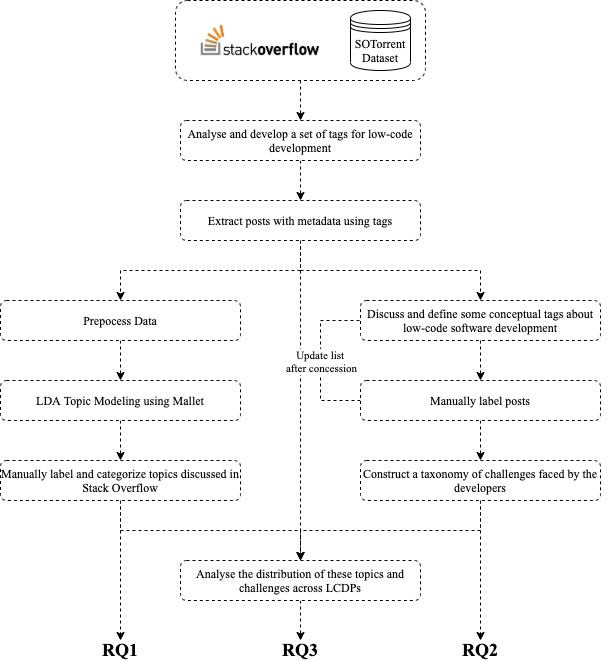
\includegraphics[width=0.35 * linewidth]{res/methology_overview.jpg}
\caption{Distribution of questions by low-code Topics (C = Customization Category, I = Integration, P = Platform Adoption, D = Database)}
\label{fig:distribution_of_questions_topic_bar_chart}
\end{figure}
\subsubsection{Results}

\begin{figure}[t]
\centering
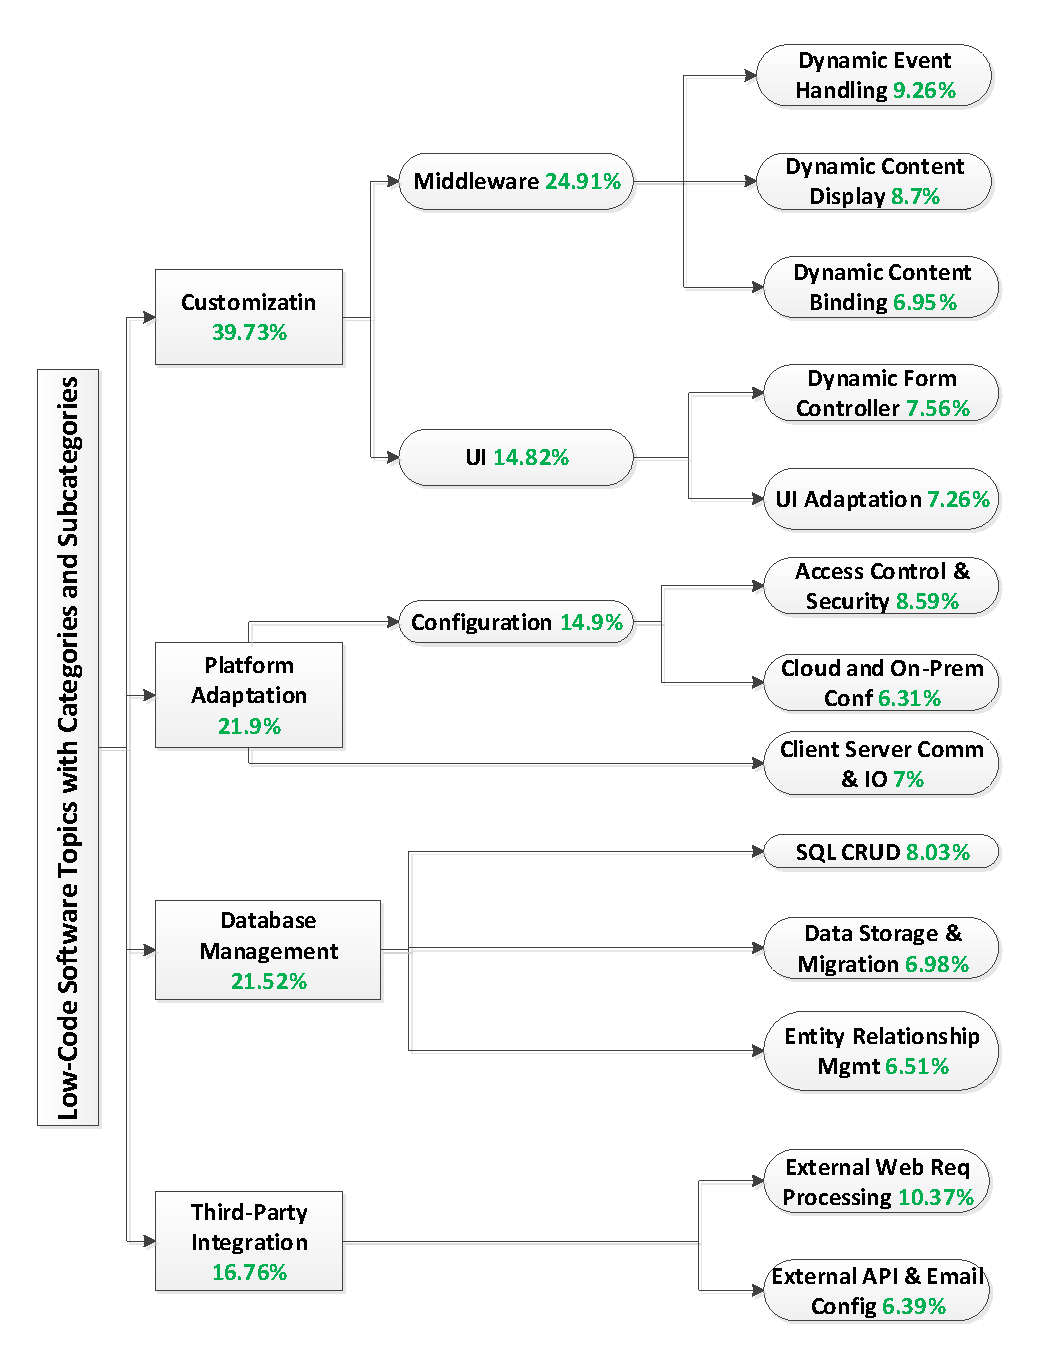
\includegraphics[scale=0.48]{res/TM_taxonomy.pdf}
% 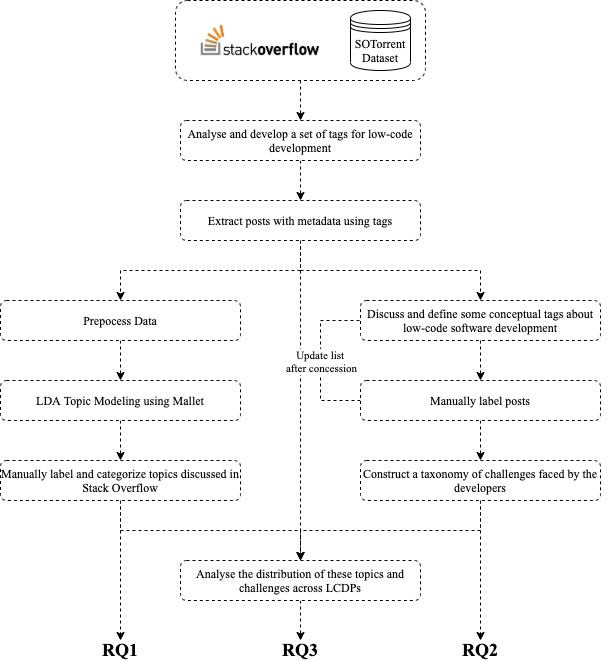
\includegraphics[width=0.35 * linewidth]{res/methology_overview.jpg}
\caption{ Low-code topics categories and sub-categories}
\label{fig:taxonomy_TM}
\end{figure}




We find 13 LCSD topics that we group into four high-level categories: \textbf{Customization, Platform Adoption, Database Management, and Third-Party Integration.} \fig\ref{fig:distribution_of_questions_topic_pie_chart} shows the distribution of
questions and topics among the four high-level categories. The \textit{Customization} category 
covers the highest percentage of questions
and number of topics (40\% questions and five topics), followed by \textit{ Platform Adoption} (22\%
questions and three topics), \textit{Database Management} (33\% questions and three topics), and \textit{Integration}
(17\% questions and two topics). \fig\ref{fig:distribution_of_questions_topic_bar_chart} sorts the 13 topics based on number of questions. The
\textit{'External Web Req Processing topic'} covers the most questions regarding queries and discussions related
to the integration of third party services/APIs (10.4\%). The \textit{'Dynamic Event Handling'} has the second most questions (9.3\%) related to the implementation of business logic.

In Figure \ref{fig:taxonomy_TM}, we group the 13 topics into four high-level categories. The categories are sorted according to the number of
questions belonging to them. For example, the topmost category \textit{Customization} has the most number of questions under them. Each category may consist of some
sub-categories. For example, \textit{Customization} Category contains two sub-categories:
\begin{inparaenum}[(1)]
\item \textit{Middleware},
\item \textit{UI}
\end{inparaenum}. Each sub-category contains one or more topics. For example,
Middleware sub-category consists of three topics: \begin{inparaenum}[(1)] \item
Dynamic Event Handling, \item Dynamic Content Display, \item and Dynamic content
Binding \end{inparaenum}. Each sub-category and topic are organized according to
their distribution of questions. For example, under Customization (40\%)
category, \textit{Middleware} (25\%) is followed by \textit{UI} (15\%) sub-category. In the same
way, 'Dynamic Event Handling' (9.3\%) topic is followed by 'Dynamic Content
Display' (8.7\%) topic based on their question distribution.



% \begin{inparaenum}[(1)]
% \item 
% \item 
% \end{inparaenum}


% \nd\bf{$\bullet$ Software Related Topics.} Out of the 40 topics, 19 topics belong to the Software category. These topics contain discussions about the 
% the usage, processing and troubleshooting of IoT software, libraries, and data. 
% The topics are grouped into three sub-categories: \begin{inparaenum}[(1)]
% \item Platform management topics contain discussions related to the IoT platforms (serivces, operating systems, SDKs, etc.),
% \item Troubleshooting topics are about the debugging of source code and the underlying IoT platforms, 
% \item Data parsing topics contain discussions about the processing of multimedia and textual contents in IoT devices.  
% \end{inparaenum} %We discuss the topics by the three sub-categories below.

\nd\bf{$\bullet$ Customization} is the largest category with 40\% of the SO posts and five topics. It contains discussions about business
logic implementation, input and form validation, linking the UI to the backend
storage via dynamic content binding, a drop-down menu with predefined value,
formatting date and time, drop-down widgets, etc. It contains two sub-categories
of topics: \begin{inparaenum}[(1)] \item \textit{UI} sub-category contains discussions
on drag-and-drop UI and form design and also customization of UI components,
\item \textit{Middleware} sub-category covers discussions on the middlewares that
provide support for system integration, the connection between UI and storage layer, etc.
%\anindya{How scalability and authentication are related to middleware is not clear. A bit of explanation would help.}
% \item Data parsing topics contain discussions about the processing of multimedia and textual contents in IoT devices.  
\end{inparaenum}

\bf{{Middleware (25\% questions)}} sub-category contains three topics:
\begin{inparaenum}[(1)] \item \it{Dynamic Event Handling (9.26\%)} has
discussions about handling user interaction events, accessing input
value after form submission (\dq{43096166}) rendering chart in the
canvas(\dq{56154215}).
%, parent component handling child component
%events(\dq{57982913}).
\item \it{Dynamic Content Display (8.70\%)} is about dynamically displaying
items on the page (\dq{53648077}), displaying content based on previous action,
creating and accessing gallery from multiple data sources (\dq{51764889}).
\item \it{Dynamic Content Binding (6.95\%)} is about updating views when some
other values get changed (\dq{59932262}) and building process based on some values
on the form (\dq{61282976}).
\end{inparaenum} 

\bf{{UI (15\% questions)}} sub-category contains two topics:
\begin{inparaenum}[(1)] \item \it{Dynamic Form Controller (7.56\%)} contains
discussions related to the design of forms with predefined values and the implementation of multi-select and customized drop-down values (\dq{44013975}), adding event-listeners to text
widget (\dq{46038130}), etc.
\item \it{UI Adaptation (7.26\%)} is about designing and customizing the user
interface using the graphical interface,
resizing console panel (\dq{34515865}).
\end{inparaenum} 

% For example, in \dq{41438021} a practitioner is about a cross origin issue and he was getting this issue because during the Ajax request the practitioners did not add the "crossOrigin: true" in the HTTP post header.

% Customization is the biggest category of topics and it contains around ?\% of documents of our topic modeling dataset. It contains four topics namely UI customization, Application customization \& Testing, Input \& form validation, Dynamic content and Data binding. The Customization category consists discussions mainly UI design and custom business logic implementation, input validation, design forms, linking the UI to the backend storage via dynamic content binding, drop-down menu with predefined value, formatting date time, drop down widgets running some basic tests. Application customization and testing topic has the highest number of average view count. Discussions in this category suggest that many practitioners lack proper programming background and task based tutorial is highly useful. For example, a practitioner is asking how to add event listener to a widget e.g., "Event Listener for App Maker Text Editor Widget" (\dq{46038130})



\nd\bf{$\bullet$ Platform  Adoption} is the second-largest category with 22\% of questions. It contains discussions about generic query on LCSD platform features
and support, role management, SDLC management tools (e.g., scrum, agile), cloud setup and configuration, deployment issues, etc. The category has three topics. One topic \it{Client Server Comm \& IO (7.09\%)} contains discussions on client-server architecture (\dq{54900592}), debugging server-side
scripts(\dq{55283256}), and general debugging queries on error messages or
unexpected output (\dq{50936643}). The other two topics are grouped under Configuration sub-category. 

\bf{{Configuration (15\% questions)}} contains discussions on LCSD platform configuration on access control and cloud-based setup. There are two topics:
\begin{inparaenum}[(1)] \item \it{Access Control \& Security (8.59\%)} is about
discussion on role-based access control to tasks (\dq{51431318}), Configuration of existing
authentication mechanism (Azure Active Directory configuration (\dq{61734680}).
\item \it{Cloud and On-Prem Conf (6.31\%)} contains discussion on the proper configuration parameters and 
guidelines to connect to the cloud/on-prem databases (\dq{55207558} \dq{45740520}).
\end{inparaenum} 



% \textbf{Platform  Adoption.}
% This high level category consists of three topics namely Platform services and Cloud configuration, Tutorial or Documentation, Deployment and Role management from our LDA modeling. Practitioners ask question on generic query on LCDPs,  what sort of features they LCDPs provide and their limitations, tutorial request on how to do a particular tasks,  cloud server configuration,  platform support on deployment and developers role management, cloud settings, different security and permission for deployment. This category consist of ?\% of total post of our dataset. Different platform provides support on version controlling, provides role management for collaborating development. Some LCDPs provides visual tools to track the progress of the application development. Some platforms also support SDLC management tools such as agile, scrum, kanban \cite{sahay2020supporting} to easy planning, tracking, and collaboration.

% % \bf{{Middleware (25\% questions)}} sub-category contains three topics: 
% \begin{inparaenum}[(1)]
% \item \ib{Dynamic Event Handling (9.26\%)} contains discussions (\dq{}), (\dq{}).
% \item \ib{Dynamic Content Display (8.7\%)} is about  (\dq{}),  (\dq{}).
% \item \ib{Dynamic Content Binding (6.95\%)} is about  (\dq{}),  (\dq{}).
% \end{inparaenum} 

\nd\bf{$\bullet$ Database} is tied to the second biggest category with 22\% of questions. It contains discussions about database connection, SQL CRUD
operations, import/export existing data, etc. There are three topics:
\begin{inparaenum}[(1)] \item \it{SQL CRUD (8.03\%)} contains discussions on SQL
query (\dq{49051500}, \dq{59852901}) and table joining(\dq{37707699}).
\item \it{Data Storage \& Migration (6.98\%)} discusses the upload
and storing of files on the server (\dq{49666940}), moving files from one platform
to another(\dq{55726281}), conversion of large CSV files to excel sheet
(\dq{50977178}), etc.
\item \it{Entity Relationship Management (6.51\%)} contains discussion on
relational database design  (\dq{51881224}) and platform support/limitations
on relational database (\dq{58935331}).
\end{inparaenum} 

% For example in \dq{34341952} a developer asking about an error while inserting new row (e.g., "Cannot insert duplicate key row in object with unique index . The duplicate key value. The statement has been terminated").


% \textbf{Database.}
% This category contains technical discussions related to backend storage design, platform support and limitation of database performance and scalability. Database is the second biggest category of topics and it contains around ?\% of documents of our topic modeling dataset. It consists of three topics namely Storage \& Data migration, Database query, and Platform support on database design. LCDPs usually connect with both SQL or NoSQL based databases. Database scalability, query optimizations, availability related complexity is abstracted from the users and in this category the discussions are more focused on how to do some CRUD operations, import/export existing data. Here a practitioner who is new to Database and low-code platform asking questions regarding how to create a duplicate value. He was getting an error because the field has unique attribute. This is a general concept in database but many of the low-code practitioners do not have strong programmatic background. "Cannot insert duplicate key row in object with unique index . The duplicate key value. The statement has been terminated" (\dq{34341952}). In this questions also asking very common database query. "SOQL - Querying for a list of users the current user is following" (\dq{9168994}).


\nd\bf{$\bullet$ Integration} around 17\% of documents and two topics. It contains discussions about email server configuration, integration
of external services, OAuth, fetching and parsing data, etc. It contains two
topics: \begin{inparaenum}[(1)] \item \it{External Web Req Processing (10.37\%)}
contains posts regarding API integration, parsing and bugging the response of
REST API (\dq{21314917}), and OAuth (\dq{56873258}), some general query on
networking protocols such as HTTP, REST API (\dq{48628269}), etc.
\item \it{External API \& Email Config (6.39\%)} is about configuration, sending
or forwarding emails (\dq{34085695}), configuration error (\dq{31501424}), how
to use generic programming language to send email (\dq{36341976}), creating
managing calendar events (\dq{46738962}), etc.
\end{inparaenum} 

% \textbf{Integration.}
% LCDPs provide developers APIs to interact with the platform and integrate different functionalities. All the challenges regarding load balancing, deploying and managing micro-services are hidden. Developers can integrate external APIs by some connectors provided by the platforms and complexities regarding authentication, security, data integrating are handled by the platforms \cite{sahay2020supporting}. The discussion on this category contains how to configure emails server, call an external API and parse the JSON response, Oath, fetch data. This category contains ?\% posts of our dataset and it contains two topics namely Email \& External Service Configuration and  General programming query and debugging external APIs. General programming query regarding API integration's has the highest number of questions and second highest number of average view counts. For example, here a developer is asking "Rest API calls with PowerApps" (\dq{37196287}). In the post the practitioner is requesting for a task based tutorial on how to make a REST API call and show the data on user interface and in the accepted answer someone suggested a tutorial post to achieve that. 
% % Discussions in this category suggests that developers lack general programming know


% \textbf{Debugging and Error:}
% In this category developers ask questions regarding different errors that they face during application development, general query on the explanation of the error code of different REST APIs, why the API is not returning expected value,  unexpected output in the console. Developers usually find the debugging quite challenging and ask different types of questions. Around ?\% questions of our dataset belong to this category. For example, here a practitioner provided a sample code and trying to debug why his method was returning undefined value e.g., "Why am I getting an undefined value when calling these scripts in Google App Maker?" \footnote{https://stackoverflow.com/questions/50936643/why-am-i-getting-an-undefined-value-when-calling-these-scripts-in-google-app-mak}. The practitioner did not understand the the sample API was async and he was supposed to use a call back method to read the response from the server.



% example of some topic and question examples
% In summary, we find that practitioners discuss on a wide range of topics including the
% limitation of LCSD platforms, how to implement complex business logic, design and scale
% up database, testing, deployment, developers' role management, dashboard, etc. 
% The developers often post queries regarding implementation issues. They also ask
% a lot of questions on general programming concepts and debugging. Our
% observation suggests that this is due to the fact that many of the low-code
% developers do not have a strong programming background and that the
% LCSD platform documentation has shortcomings.


\begin{tcolorbox}[flushleft upper,boxrule=1pt,arc=0pt,left=0pt,right=0pt,top=0pt,bottom=0pt,colback=white,after=\ignorespacesafterend\par\noindent]
\noindent\textbf{Summary of RQ1. What topics are discussed by low code
developers in SO?} We found 13 topics in our SO dataset relevant to low-code
software development.  The topics belong to four categories: Customization,
Platform Adoption, Database, and Integration. Customization category has the
most number of questions, followed by Platform Adoption, Database, and
Integration. Out of the topics, `External Web Request Processing' topic under
the Integration category constitutes the highest number of questions (10.4\%)
followed by the topic `Dynamic Event Handling' (9.3\%) under the Customization
category.
\end{tcolorbox} 







\subsection{How do the topics distribute across low-code SDLC? (RQ2)}\label{sec:rq-topic-challenges}


% \subsubsection{Motivation} 
% % motivate why this research question is important

%  In traditional agile software development approach a application usually goes through six phases. LCSD platforms provides many features to reduce the complexities related to server settings, scalability, performance issues that practitioners usually face during traditional software deployment and maintenance phase \cite{sahay2020supporting}. From our RQ1, we find that practitioners ask different questions from requirement \& feasibility analysis to application development to testing-deployment. In this research question, we investigate the challenges developers face at different phases of SDLC. This will provide a valuable insight  to the future researchers and low-code platform providers to understand and improve their platforms. 


\subsubsection{Approach}
%Previous studies \cite{rosen2016mobile}\cite{abdellatif2020challenges} show that developers ask different types of questions (i.e., How, what, why) to express the challenges they are facing. 
%As we noted in \sec\ref{sec:background}, LCSD development phases can have some subtle differences (e.g., shorter length) from traditional software development phases. 
Agile software development methodology~\cite{beck2001manifesto} has six SDLC phases:  \begin{inparaenum}[(1)]
\item Requirement Analysis \& Planning, 
\item Application Design,
\item Implementation, 
\item Testing,
\item Deployment, and
\item Maintenance 
\end{inparaenum}. We manually label 900 randomly sampled questions as one of these six development phases. For each question, we read its description and the provided answers (with a non-negative score) to fully understand the exact development phase. For example, a new practitioner is tasked with finding the right LCSD platform during the planning stage of his/her 
LCSD application. The practitioner queries ``Are there any serious pitfalls to Outsystems Agile Platform?" (\dq{3016015}). We thus assign the SDLC phase for it as `Requirement Analysis \& Planning'. Another question asks ``Google  App  Maker  app  not  working  after  deploy" (\dq{42506938}). We label the SDLC phase as 'Deployment'. 


\begin{figure}[t]
	\centering
	\resizebox{2.8in}{!}{
	\begin{tikzpicture}%[scale=0.34]-
    \pie[
        %/tikz/every pin/.style={align=center},
        %text=pin, number in legend,
        %explode=0.0,
        explode=0.0, text=pin, number in legend, sum = auto, 
        color={black!10, black!20, black!0, black!30,black!40},
        ]
        {
            1.4/\Huge{Testing}1.4\%,
            2.5/\Huge{Deployment} 2.5\%,
            87/\Huge{Implementation} 87\%,
            1.5/\Huge{Req Analysis} 1.5\%,
            4.5/\Huge{Design} 4.5\%,
            2.6/\Huge{Maintenance} 2.6\%
        }
    \end{tikzpicture}
    }
	\caption{Distribution of questions (Q) per SDLC phase}
	%\vspace{-5mm}
	\label{fig:distribution_of_SDLC_pie_chart}
\end{figure}
\begin{table}[t]
  \centering
  %\vspace{-.1in}
   \caption{Distribution (frequency) of LCSD topics per SDLC phase. Each colored bar denotes a phase 
   (Black = Requirement Analysis \& Planning, Green = Application Design, Magenta = Implementation, Red = Testing, Blue = Deployment, Orange = Maintenance)}
  % \vspace{-3mm}
    \resizebox{\columnwidth}{!}{%
    \begin{tabular}{lr}
    \toprule{}
    % \textbf{Topics} & \textbf{Authentication} & \textbf{Deployment} & \textbf{Documentation} & \textbf{Feature} & \textbf{Testing/Debugging}\\
    \textbf{Topics} & \textbf{Development Phases Noted in \#Questions}\\
    \midrule
    \textbf{Customization (351, 39\%)} &  \\
    Dynamic Event Handling	& \sixbars{0}{0}{73}{7}{1}{0}		\\
    Dynamic Content Display & \sixbars{0}{2}{78}{1}{0}{0}	\\
    Dynamic Form Controller	& \sixbars{0}{2}{67}{0}{0}{0}	\\
    UI Adaptation	& \sixbars{0}{1}{59}{1}{1}{2} \\
    Dynamic Content Binding	& \sixbars{0}{5}{49}{0}{0}{2} \\
    \midrule
    \textbf{Platform Adoption (189, 21\%)} &  \\
    Access Control \& Security	& \sixbars{4}{3}{42}{2}{14}{12} \\
    Client Server Comm \& IO	& \sixbars{0}{0}{54}{2}{1}{0}  \\
    Cloud and On-Prem Conf & \sixbars{8}{12}{28}{1}{4}{2} \\
    \midrule 
    \textbf{Database (214, 23.7\%)} &  \\
    SQL CRUD	& \sixbars{1}{4}{74}{0}{0}{0} \\
    Data Storage \& Migration	& \sixbars{0}{3}{63}{0}{0}{2} \\
    Entity Relationship Mngmt	& \sixbars{1}{5}{58}{0}{0}{3} \\
    \midrule
    \textbf{Integration (145, 16.1\%)} &  \\
    Ext Web Req Processing & \sixbars{0}{3}{99}{0}{0}{0}	\\
    Ext API \& Email Config & \sixbars{0}{0}{41}{0}{1}{1}\\
    \bottomrule
    \end{tabular}%
   }
   % \vspace{-.25in}
  \label{tab:topicSDLC}%
\end{table}%



%\gias{Please review first paragraph}
\subsubsection{Results} Figure \ref{fig:distribution_of_SDLC_pie_chart} shows that Implementation phase is found in 85\% of the 900 questions we studied, followed by Maintenance (2.6\%) and Deployment (2.4\%) phases. This is not surprising, given that SO is a technical Q\&A site and developers use the forum to find solutions to their technical problems. Table \ref{tab:topicSDLC} shows the distribution of our 13 LCSD topics over six low-code SDLC phase base on our analysis of 900 SO questions. Besides the dominance of development phase related questions across all topics, we find the presence of other phases (e.g., testing, development) in customization and platform adoption topics. 

% \textbf{ Irrelevant Tag(16, 1.6\%) } While labelling questions from our dataset $B$ we found that there were some questions has been tagged with a low-code platform tags but it does not contain any issues related to LCSD, rather these are generic software technology related queries or queries about some low-code application configuration (specially Zoho email service). For example, In \dq{18335697} a pratitioner is trying to send email using Zoho email service (e.g., "Send email through Zoho SMTP" "Zoho Mail" with tag "zoho").  Another example is in (\dq{54113212} a practitioner is asking about "How to reference resource file in java maven project running in docker container". It does not contain discussion related to LCSD.

% \textbf{ Authentication \& Authorization (37, 3.7\%)} It contains technical challenges related to  Application access control (CORS) policy, permission related to deployment, Social authentication, IAM role management (\dq{42841546)} etc. 
% \textbf{ Deployment (18, 1.7\%).} It contains technical challenges about deployment issues (\dq{46369742}), sharing public URL of the application(\dq{44136328}), custom domain name or URL, etc. Sometimes practitioners make a general query on deployment (e.g., \emt{"How can I share my app made by Google App Maker with others?"}\dq{44025410} ).

% \textbf{ Documentation (201, 20.1\%)} It is the second biggest technical challenge. It contains discussions related to how to do or find documentation/tutorial for a particular task of platform features, integrating external services, database query and connection, UI design etc. The root cause of these issues are incomplete or incorrect documentation. In \dq{46241015} a practitioner is querying integration of Zoho CRM and says he does not understand the sample code. The question has 2 up-votes, so it seems like other practitioners also find the documentation difficult to understand. In \dq{34510911} a practitioner is asking "Html2PdfConverter Sample Conversion". Here a new LCSD practitioner is asking about sample code to convert a web page to a PDF.

% \textbf{ Feature (543, 54.2\%)} It is the biggest category of challenges that contains challenges on general queries on LCSP platform and its features and limitation on UI design (\dq{40159662}), data modelling, customization, community support etc. A big portion of queries are related to platform support of data storage, database connection and query \dq{9168994}. For example in \dq{34341952} a developer asking about an error while inserting new row (e.g., "Cannot insert duplicate key row in object with unique index . The duplicate key value. The statement has been terminated").

% \textbf{ Testing/Debugging (187, 18.7\%)} It contains challenges related to debugging i.e, input output mismatch, error, unexpected output, and on testing i.e., how to run tests, test coverage, issues using third party functional testing tools like Selenium (\dq{61210424}) etc. Most of these challenger arise during application development and testing phase while practitioners want to implement custom business logic. For example, In \dq{12412269} a practitioner is asking about an error message while making a XML request in PHP. 

% \textbf{ Irrelevant Tag(16, 1.6\%) } While labelling questions from our dataset $B$ we found that there were some questions has been tagged with a low-code platform tags but it does not contain any issues related to LCSD, rather these are generic software technology related queries or queries about some low-code application configuration (specially Zoho email service). For example, In \dq{18335697} a pratitioner is trying to send email using Zoho email service (e.g., "Send email through Zoho SMTP" "Zoho Mail" with tag "zoho").  Another example is in (\dq{54113212} a practitioner is asking about "How to reference resource file in java maven project running in docker container". It does not contain discussion related to LCSD.


% \paragraph{Distribution of Technical Challenges per Low-code Topic.}

% Table \ref{tab:challengespertopic} shows that Customization is the biggest category that contains around 38\% of technical challenges. 

% \paragraph{Taxonomy of practitioners' challenge}
% Practitioners ask different questions from requirement \& feasibility analysis to application development to testing-deployment. Fig. \ref{fig:taxonomoy_low_code_challenges} shows the hierarchical taxonomy of different issues that low-code developers face during different phases of the agile low-code development life cycle. The taxonomy is organized into six major categories corresponding to the agile development life cycle phases. We created this taxonomy after carefully analyzing the questions discussed in SO and then we used the bottom-up approach to group the queries into sub-categories or sub-sub-categories based on the challenges faced by the developers. Some group of queries like platform features and limitations, tutorial request on API usage, and external service integration, data migration arise in different phases of agile SDLC. Fig. \ref{fig:taxonomoy_low_code_challenges} shows, most of the questions (?\%) are asked during the application development life cycle. ?, ?, ? has the highest number of questions. 


% \paragraph{Distribution of topics across different software development phases.}
% Practitioners ask different questions from requirement \& feasibility analysis to application development to testing-deployment. Agile software development methodology\cite{beck2001manifesto} has mainly six development phases:  \begin{inparaenum}[(1)]
% \item Requirement Analysis \& Planning, 
% \item Application Design,
% \item Implementation, 
% \item Testing,
% \item Deployment, and
% \item Maintenance 
% \end{inparaenum}. Table \ref{tab:challengesperSDLC} shows the distribution of technical challenges distribution into six major categories corresponding to the six development phases of agile software development life cycle phases. We created this table after carefully analyzing the questions discussed in SO. Some technical challenges like Features that contains challenges on platform features and limitations, tutorial request on API usage, and external service integration, data migration arise in different phases of agile SDLC. Table \ref{tab:challengesperSDLC} shows, most of the questions (85\%) are asked during the application development life cycle followed by Deployment and Maintenance phase. 

\bf{Requirement Analysis \& Planning (14, 1.5\%).} 
Requirement analysis is the process of developing software according to the expectation of the users. 
% The business requirement is dependent on the goals and visions of the business.
During planning, the feasibility, timeline, dependability, potential complexity/risks are analyzed and planned by paying attention to the operational aspects. The LCSD platforms usually provide requirement management tools that allow developers to collect data, customize checklists, import user stories into sprint plans. At this phase, the developers usually face enquiries about cost, learning curve, LCDP's support for faster application development, deployment, and maintenance features to choose the right platform for their business need. For example, In this popular question, a new practitioner is asking for some drawbacks on some potential pitfalls for a particular LCDP, e.g., "Are there any serious pitfalls to Outsystems Agile Platform?" (\dq{3016015}). A developer from that platform provider suggests using the platform to build an application and decide for himself as it is hard to define what someone might consider a pitfall. 

% The discussion in this questions was closed  because SO community guideline mandates its discussion should focus on specific questions rather than general broad discussion. Practitioners also query like this "Looking for education materials about App Maker" (\dq{55304547}) and query about learning curve.

% The success of software development largely depends on the successful capture and management of application requirements and planning accordingly. 

% What are people's experiences with these online DB apps? Should I keep pushing ahead, or just write a custom app myself?
% Do apps built with AppMaker scale?
% Does Mendix generates a source code in any particular language, which can be edited and reused? I have never used Mendix
% Why should i choose a webservice versus adding the logic to mobile code? Salesforce web versus iOS Native App
% I made some customization in Zoho CRM module and now I want to reuse these customization in another Zoho CRM
% Can anyone suggest how can we represent the architecture of app maker

% project failure
% choose new platform
% reputation
% defeats the whole purpose



\bf{Application Design (40, 4.5\%).} In this phase, the design specification is made based on the requirements of the application. All the key stakeholders review and approve this considering application architecture, modularity, extensibility. The LCSD developers face challenges regarding data storage design, drag and drop UI design, using on-prem data-sources with the LCSD platform (e.g., "Can AppMaker be used with SQL Server" (\dq{55220499})), migrating existing data to LCSD platform (\dq{46421271}), designing a responsive web page (e.g., "Incorporating responsive design in App Maker" (\dq{52744026})).

% Developers asking how he can reuse one menu page across the whole application. "How to create header menu for multiple page in powerapss?" \footnote{https://stackoverflow.com/questions/56213578/how-to-create-header-menu-for-multiple-page-in-powerapss}
% Data migration tools to migrate exisiting unstructure data to a SQL based datastorage. "Convert Sharepoint List into structured database" \footnote{https://stackoverflow.com/questions/61379667/convert-sharepoint-list-into-structured-database}
% How to create a basic dropdown list with  some reference item.
% "Power apps drop down" \footnote{https://stackoverflow.com/questions/41806580/power-apps-drop-down}

\bf{Implementation (785, 87.3\%).} At this phase, actual application development begins. LCSD developers face a wide range of challenges when they try to customize UI, implement business logic, integrate third-party modules, debug and test the implemented functionalities, read the incomplete or incorrect documentation, etc. Developers ask application customization and UI customization questions like "How do I change timezone in AppMaker Environment?" (\dq{47731051}), drop-down menu customization (e.g., "powerapps: populate drop down list from another datasource" (\dq{40159662})). There are many queries (17\%) regarding external services or API integration. Many of these questions are relevant to a task-based tutorial on how to use a REST API and process its response (e.g., "How to upload files and attachments to the subject record using REST API?" (\dq{61143493})). The root cause of many of these issues is incomplete or incorrect documentation. For example, In \dq{46241015}, a practitioner is querying about the integration of Zoho CRM and says that s/he does not understand the sample code. In \dq{34510911}, a practitioner asks for sample code to convert a web page to a PDF. Clearly, the documentation is not sufficient for a smooth transition for entry-level practitioners.
%"Html2PdfConverter Sample Conversion". Here a new low code practitioner is asking about sample code to convert a web page to a PDF.


% asking general questions on how to LCDP to other services. "Sending Images from PowerApps to Microsoft Flow" \footnote{https://stackoverflow.com/questions/41577382/sending-images-from-powerapps-to-microsoft-flow}




% Google Domain, Zoho Email, MailGun Delivery: SPF Entries error
% OmniScript Designer Javascript and HTML css customization in Vlocity
% The onbeforeunload event does not occur when the browser tab of appmaker web app closes
% MisFit API inegration not supporting in Outsystem InAppBrowser
% PowerApps Date picker control - how to set minDate and maxDate range
% Does PowerApps Feature support Cross-Site Lookup in SharePoint - Getting Error Creating App from Data
% How to retrieve FeedComment using Chatter SalesForce WSDL service in C#
% Create calendar Event in Google App maker

% How can I show a PowerApp in VSTS / Azure Devops dashboard?
% How can I show a PowerApp in VSTS / Azure Devops dashboard?
% Best practice
% implement funtionalities
% extend in the future



\bf{Testing (14, 1.5\%).} % https://bitbar.com/blog/low-code-development-what-why-and-how-does-it-impact-testing/
The testing process of LCSD varies from traditional software. It usually takes less testing LCSD platforms because the platform management team test and monitors the modules provided. Unit testing carries less importance than tradition development because the components are already unit tested, and developers usually integrate those using drag-and-drop fashion. Many platforms provide custom unit testing features for the application logic code added by the developers. The platform providers recommend to run a security audit to check if there is a potential data exposure. Most of the issues faced in this phase are related to browser compatibility, lack of proper documentation to run automated tests, test coverage, issues using the third party functional testing tools like Selenium (\dq{61210424}), etc. Practitioners make general queries about running tests on low code platforms (\dq{46669690}), errors while running test (\dq{47254010}).

% It contains challenges related to debugging i.e, input output mismatch, error, unexpected output, and on testing i.e., how to run tests, test coverage, issues using third party functional testing tools like Selenium (\dq{61210424}) etc. Most of these challenger arise during application development and testing phase while practitioners want to implement custom business logic. For example, In \dq{12412269} a practitioner is asking about an error message while making a XML request in PHP. 


% Google app maker testing approach
% “Unexpected token import” when testing Angular with Jest
% What can cause a user to be able to only see one row in a report? Browser issue?
% LWC test using jest testing framework throws error - unknown public property "smalldevicesize" of element
% How to test a PowerApps Custom Connector GET request at localhost?
% Code Coverage Failure Your code coverage is 72%. You need at least 75% coverage to complete this deployment

% reliability security is compromised

\bf{Deployment (22, 2.5\%).} LCSD platforms aim to make \textit{deployment and maintenance} phase smooth. Many platforms provide Application Life-Cycle Management tools to develop, debug, deploy, and maintain the staging and production server application. However, LCSD developers still face challenges regarding deployment configuration issues (\dq{46369742}), version control, DNS configuration, performance issues, accessibility issues (i.e., sharing public URL of the application (\dq{44136328}, \dq{53884162})), DNS configuration etc. For example, in this discussion, a developer was having trouble in accessing the app after deployment (e.g., "Google App Maker app not working after deploy" (\dq{42506938})). In the accepted answer, a community member provides a detailed description to achieve that and points out the lack of \textit{Official documentation} for such a crucial task. There are a few queries about deploying application with custom URL i.e. domain name (E.g., "How to make friendly custom URL for deployed app" (\dq{47194231})). In this case, it was difficult because the platform did not have native support. 
% "If a user is not an Admin, he can't access application". \footnote{https://stackoverflow.com/questions/46495006/if-a-user-is-not-an-admin-he-cant-access-application}

% It contains technical challenges about deployment issues (\dq{46369742}), sharing public URL of the application(\dq{44136328}), custom domain name or URL, etc. Sometimes practitioners make a general query on deployment (e.g., \emt{"How can I share my app made by Google App Maker with others?"}\dq{44025410} ).


% Here a developer is making general query regarding if a particular SDLC supports multiple domain where he can provide SAAS service to multiple clients "Deploying AppMaker app on multiple domains" \footnote {https://stackoverflow.com/questions/41467659/deploying-appmaker-app-on-multiple-domains}
% Developers ask questions like "

% Google App Make: Unable to choose Cloud SQL option for deployment
% Written Very Basic APEX Class, How Can my Customers get to access it?
% How to access to Reachability in MKNetworkKit-iOS or avoid duplicate symbols with own added Reachability?
% How to version control PowerApps project in DevOps repo \footnote{https://stackoverflow.com/questions/60159719/how-to-version-control-powerapps-project-in-devops-repo}
% Not able to add custom domain in Salesforce

% citizen developer server admin
% difficult to fix issues



\bf{Maintenance (24, 2.6\%).} At this stage, the application is released and needs maintenance support. The users sometimes find bugs that were not caught before and sometimes want new features that may spawn a new software development life cycle in agile or incremental development methodology. In this phase, developers face challenges regarding bugs in a low-code platform and difficulties in using different application maintenance features provided by the platform such as event monitoring, collaboration, application design reusability, etc. Different LCSD platforms provide features on developers' role management, dashboard, and event monitoring. For example, in this question a practitioner queries about the feasibility of role-based access control in an LCSD platform: "PowerApps : Implementing Role Based Security In Your PowerApps App" (\dq{52762374}). LCSD developers also find it difficult to determine/update versions of LCSD platforms (see \dq{45209796}). 
%An LCSD developer asks "Do I have the latest version of an OutSystems forge component?" (\dq{45209796}). 


% \paragraph{Root cause of difficult challenges practitioners face}
% 
% % This change in design creates some challenges for developers during development phase because sometimes the customization requires some features that is not supported by the platform or requires in depth understanding of the platform.
% The most difficult challenges the practitioners face are because of the higher level of abstraction and platform limitations. Using low code platforms business applications can be developed by the people who will use the system. It enables business people to rapidly create necessary business application that adds value to the organization. Low-code development platform provides a high level abstraction of UI design by drag-and-drop interface, managing data storage, data integrity, load balancing, authentication and security. This abstraction enables practitioners to develop fully functional business applications with very little written coding. This works as a two way sword because 
% if a practitioner needs to implement a complex customization, he sometimes does not know how to approach the problem because, he is not aware of the complexity of auto generated codes, database connection and CRUD operation etc. It requires in depth knowledge about the platform and if the documentation or sample examples API usage does not cover it, the practitioners keep on asking for tutorials on how to do achieve this. This is a difficult problem even for experienced software engineers, considerably more the less experienced low-code practitioners.
% 
% Another big issue is Platform limitations. Usually at the beginning of the project the developer teams chooses a low-code platform that satisfies their business requirement. But in Agile and incremental development methodology, the business the features are implemented incrementally and sometimes the business requirements changes and wants additional functionalities.  Platform limitation questions raises because the business requirement of the application changes and if the platform does not provide a easy way to implement that feature  and then the developers find the situation most challenging.

% Zoho Recruit API redirecting to their homepage   // mistake
% Viewer access to Dashboard folders
% If a user is not an Admin, he can't access application
% How do perform logging or debug output in a server script?
% SubmitForm is not working in power apps  // bug
% Security measures between appmaker and Google Cloud SQL
% PowerApps : Implementing Role Based Security In Your PowerApps App  // role management
% hard to add new features
% maintain reputation


\begin{tcolorbox}[flushleft upper,boxrule=1pt,arc=0pt,left=0pt,right=0pt,top=0pt,bottom=0pt,colback=white,after=\ignorespacesafterend\par\noindent]
\noindent\textbf{Summary of RQ2. How do the topics distribute across low-code SDLC?} We 
randomly sampled 900 questions from our dataset and manually examined the type of SDLC phase for which the developer asked the question. We found an overwhelming majority of (85\%) implementation phase related questions in SO. Non-coding questions are generally discouraged in SO. We find few questions related to other phases (e.g., requirement analysis, deployment, etc.). We also find that LCSD developers find testing is challenging for LCSD application due to the graphical nature of the SDKs, which can be hard to debug.
\end{tcolorbox}


\subsection{What LCSD topics are the most difficult to answer? (RQ3)}\label{sec:rq-topic-difficulty}

\begin{table*}[t]
  \centering
  %\vspace{-.1in}
   \caption{Low-code software development topics, their popularity, and difficulty}
  % \vspace{-3mm}
 % \resizebox{\columnwidth}{!}{%
    \begin{tabular}{llrrrrrrr}
    % \begin{tabular}{m{16em}m{6em}m{3.3em}m{2.5em}m{2.5em}m{3em}m{3em}m{4.5em}m{4em}}
    \toprule{}
    \multirow{2}{*}{\textbf{Topic}} & \multirow{2}{*}{\textbf{Category}} & \multicolumn{4}{c}{\textbf{Popularity score}} & \multicolumn{3}{c}{\textbf{Difficulty score}} \\
    \cmidrule{3-9}
    {} & {}  & \textbf{Avg view} & \textbf{Avg fav.} & \textbf{Avg score} & \textbf{Avg \#ans} & \textbf{W/O any ans.} & \textbf{W/O acc. ans.} & \textbf{Med. Hrs acc.} \\
    \midrule

   Dynamic Event Handling	&	Customization &	833 &	1.23 &	0.54 & 0.86	& 37.2\% & 75.9\% &	9.8 \\
   Ext. Web Req Processing & Integration & 785 &	1.24 &	0.62 & 1.04	& 23.3\% &	68.1\% &	15.7 \\ 
   Ext. API \& Email Config &		Integration &	764 &	1.23 &	0.83 &	0.91 &	34.3\% & 70.4\% &	12.7 \\
   Dynamic Content Display &	Customization 	& 722 &	0.86 & 0.48 & 0.99 &	17.6\%	& 65.2\%	& 14.8 \\
   Cloud and On-Prem Conf	&	Adoption &	578 &	1.18 &	0.85 & 1.01 &	23.8\% &	66.5\% &	16.8 \\  
   Dynamic Form Controller	&	Customization  &	566 &	0.85 &	0.45 & 1.07	& 15.1\% &	57.4\% &	4.2 \\
    UI Adaptation	&	Customization  &	536 &	0.95 & 	0.46 & 0.88 &	30.3\%	& 68.2\% &	6.1 \\ 
    Dynamic Content Binding	&	Customization &	507 &	1.16 &	0.36 & 0.94	& 22.4\% &	67.2\% &	24.9 \\
   Entity Relationship Mngmt	&	Database &	485  &	1.09 &	0.48 &	0.93 &	29.5\% & 62.4\% &	6.9 \\  
    Data Storage \& Migration	&	Database &	472 &	1.07 &	0.60 & 0.89 &	25.1\% &	69.3\% &	14.8 \\
    Client Server Comm \& IO	&	Adoption &	408	& 1.11 &	0.54 & 0.86	& 31.8\% &	67.8\% &	12.7 \\ 
    SQL CRUD	&	Database	& 359 &	1.04 &	0.45 & 0.92 &	22.1\%  &	60.2\% &	7.6 \\
   Access Control \& Security	&	Adoption &	301 &	0.97 &	0.49 & 0.93 &	26.2\% & 69.9\% &	12.6 \\
    \midrule
    \multicolumn{2}{l}{\textbf{Summary}}  & \textbf{572} & \textbf{1.1} & \textbf{0.5} & \textbf{0.9} & 26\% &\textbf{67\%} & 12.3 \\
    \bottomrule
    \end{tabular}%
   % }
   % \vspace{-.25in}
  \label{tab:topicPopularityDifficulty}%
\end{table*}%

\begin{table}[t]
  \centering
  \caption{Correlation between the topic popularity and difficulty}
    \begin{tabular}{lrrr}\toprule
    coefficient/p-value & \bf{View} & \bf{Favorites} & \bf{Score}\\ \midrule
    \bf{\% without acc. ans.} &   0.154/0.51    & 0.348/0.10      &  0.379/0.08 \\
    \bf{Hrs to acc. ans.} &    0.077/0.77   &   0.400/0.06     & 0.431/0.04  \\
    \bf{\% without any answer} &   0.077/0.77    & 0.374/0.08      &  0.275/0.20 \\
    \bottomrule
    \end{tabular}%
   % \vspace{-.2in}
  \label{tab:correlation}%
\end{table}

% Pct_Questions_without_Accepted_Answer Averege_View 0.154 0.51 False
% Pct_Questions_without_Accepted_Answer AVerege_Favorite 0.348 0.10 False
% Pct_Questions_without_Accepted_Answer Averege_Score 0.379 0.08 False
% Median_Hours_To_Get_Accepted_Answer Averege_View 0.077 0.77 False
% Median_Hours_To_Get_Accepted_Answer AVerege_Favorite 0.400 0.06 False
% Median_Hours_To_Get_Accepted_Answer Averege_Score 0.431 0.04 True
% PcWithOutAns Averege_View 0.077 0.77 False
% PcWithOutAns AVerege_Favorite 0.374 0.08 False
% PcWithOutAns Averege_Score 0.275 0.20 False

% \subsubsection{Motivation} 
% Our findings from the above two research questions show that LCSD developers 
% face challenges more unique to LCSD platforms (e.g., customization topics) as well as similar to other domains (e.g., database topics). Therefore, 
% it can be userful to learn what topics are more difficult to get the right answer to and whether the popularity of the 
% topics can suffer due to the observed difficulty.

\subsubsection{Approach} For each topic, we compute the difficulty of getting answers under a topic using three metrics: \begin{inparaenum}[(1)] \item Percentage of questions without an accepted answer,
\item Average median time needed to get an accepted answer,
\item Percentage of questions without any answer at all.
\end{inparaenum} In the same way we use the following four popularity metrics: \begin{inparaenum}[(1)]
\item Average number of views, \item Average number of favorites, and \item Average
score, and \item Average number of answers \end{inparaenum}. Then we aim to determine the correlation between difficulty and
popularity of the topics. The first two difficulty metrics and first three popularity metrics are used in several previous studies~\cite{bagherzadeh2019going, abdellatif2020challenges, ahmed2018concurrency}. We use Kendall Tau correlation measure~\cite{Kendall-TauMetric-Biometrica1938} to
find the correlation between topic popularity and topic difficulty. SO does not
provide the data across a time-series for all metrics such as view count, score etc. As such, our analysis offers as of time insight. 
%Hence, our analysis on topic difficulty and popularity can only provide
%insights on current low-code related discussions.

\subsubsection{Results}
Table \ref{tab:topicPopularityDifficulty} shows the topic difficulty using the three metrics, as noted above. 
These two metrics allow us to find the difficulty to get a solution that works ~\cite{bagherzadeh2019going} and \cite{abdellatif2020challenges}. 
The \textit{Dynamic Event Handling} under Customization has the highest average view count and the highest percentage of questions (76\%) without an accepted answer. \textit{Dynamic Content Binding} from the same category also has the highest median hours to get an accepted answer. Many questions in this topic relate to business logic customization in a LCSD platform, which is not familiar to other developers. For example, \dq{51443599} asks "How to add more data an array of objects in a lightning component?". This question has been asked around two years ago, viewed around 11K times and still active. It has three answers, but none of them is marked as accepted. On the other hand, \textit{Dynamic Form Controller} under Customization is the least difficult topic concerning the percentage of the question without an accepted answer (57\%) and median time (4.2 hours) to get a solution. It is because questions related to form design and validation are common and have good \textit{community support}. Same is also true for the topic \textit{SQL CRUD} which has around 7.6 median hours for accepted answers.

The \textit{External Web Req Processing} under
 \textit{Integration} has the highest percentage of questions and highest average
favorite count. The \textit{Cloud and On-Prem Conf}
under  \textit{Platform} adoption has the highest average score. The
discussions are about setting and maintaining cloud configuration and migrating
on-prem data to the server in this topic. For example, \dq{44727285} a practitioner is asking
about  "Migrate Salesforce data from one org to another", and in \dq{3016015}, a
new practitioner is making a general low-code platform related to query "Are
there any serious pitfalls to Outsystems Agile Platform?". This question has
very high score because lots of new low-code platform developers have faced this
issue. \textit{Access Control \& Security} under Platform Adoption is the least
popular topic in terms on average view count. Here the questions are about
deploying the application, its security and access control. For example, in
\dq{17886545} a practitioner says "Can't Connect to SalesForce in C\#". He also
explains there is a security token error and in the documentation its not
mentioned how to configure that. Many of these questions are not general, and
so it has a low average view-count.

\nd\textbf{Correlation between topic difficulty and popularity.} 
In Table \ref{tab:correlation}, we present nine
correlation measures using three difficulty and popularity metrics from Table
\ref{tab:topicPopularityDifficulty}. Our result shows no
statistically significant correlation between the popularity and difficulty
metrics since for eight out of nine correlation values are \textgreater~0.05. Therefore, we cannot say that the least popular topics are the most difficult
ones and vice versa. For example, Access Control \& Security is one of
the least popular topics, but considered among the most difficult topics (Table
\ref{tab:topicPopularityDifficulty}). However, this observation does not hold for
topic Dynamic Event Handling, which is the most popular and among
the most difficult topics.  

% (Sir) However, the correlation measures are not at 95 percent confidence labal (statistically significant)
% This finding can provide insights to low-code platform developers and educators to reduce the difficulty labels of the topics.

\begin{tcolorbox}[flushleft upper,boxrule=1pt,arc=0pt,left=0pt,right=0pt,top=0pt,bottom=0pt,colback=white,after=\ignorespacesafterend\par\noindent]
\noindent\textbf{Summary of RQ3. What LCSD topics are the most difficult to answer?} We compute seven popularity and difficulty metrics for each topic using metrics such as  
view count, percentage of questions without an accepted answer etc. We find that questions related to topic ``Dynamic Event Handling'' from the 
customization category are the most difficult (to get an accepted answer) but also the most popular (average view count). Overall, we do not see any significant correlation (positive/negative) between topic difficulty and popularity metrics. 
\end{tcolorbox}
